In this section, we present the analysis of schemes introduced in the above sections. The analysis is divided in to two parts: the first part presents a tabular format of the benefits and cost for each of the sub-scheme. In the second section, we present the performance results obtained by processing the address traces shared by Huawei. \\ 
Table~\ref{table:benefit_cost} presents the benefits and cost of each of the sub-scheme. It essentially presents the summary of the analysis done in the previous sections where we introduced each of these schemes. The condensed tabular format can be used to compare the cost and benefits of each of the sub-schemes. 
\begin{comment} 
\begin{figure}[ht!]
\centering
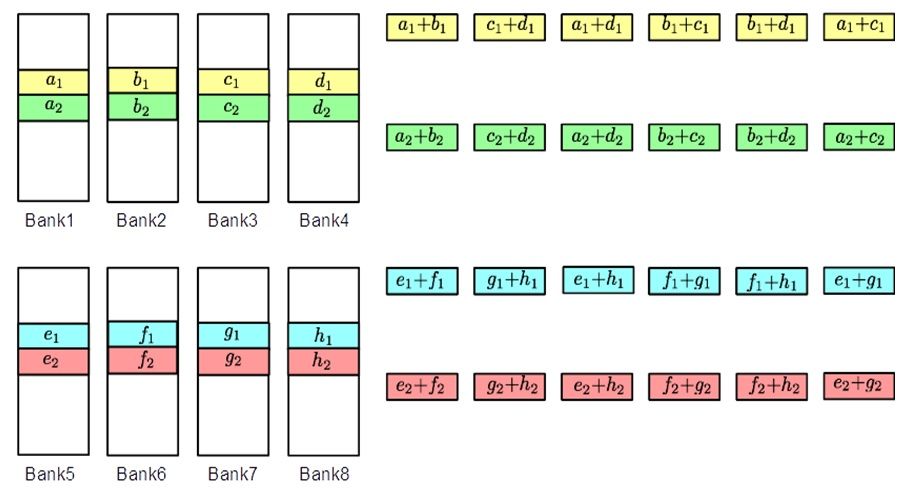
\includegraphics[width=450pt,natwidth=908,natheight=488]{code_region.jpg}
\caption{Memory Bank layout}
\label{fig:code_region}
\end{figure}
\end{comment}
\begin{table}[ht!]
    \begin{tabular}{ | p{2cm} | p{7.5cm} | p{7.5cm} |}
    \hline
    Sub Scheme & Benefits (Per Region) & Costs \\ \hline
    Memory Coding &
    \vspace{-7mm}  
    \begin{itemize} 
    \item 10 reads Best case 
    \item 7 reads worst-worst case
    \item 2 writes per bank so 8 writes per region. Both for best case and worst case.
    \end{itemize}
    & 
    \vspace{-7mm} 
    \begin{itemize} 
    \item 1.5$\alpha$ times more memory.  
    \item control logic overhead for doing parallel reads and writes.
    \item Overhead of re-coding after a write. Each write needs a 3 reads and 4 writes.  
    \end{itemize}
 \\ \hline
    Dynamic Coding & 
    \vspace{-7mm} 
    \begin{itemize}
    \item Reduces the memory overhead to 5$\%$
    \item Makes $\alpha$ to be 
    \end{itemize}
    & 
    \vspace{-7mm} 
    \begin{itemize}
    \item Control logic for doing dynamic allocation. 
    \item Overhead of recoding during change of coded region. 
    \end{itemize}
 \\ \hline 
    Prefetching the codes & 
    Benefits more efficient reads & 
    Control logic for looking ahead in memory queue to prefetch the codes. 
 \\ \hline
    \end{tabular}
    \caption{Cost and Benefit of Coding scheme}
    \label{table:benefit_cost}
\end{table}
\\
Figure

\subsection{Simulation Setup}
\label{sec:simulation_setup}
Coding the memory banks to help extra accesses requires the scheme to be 

